\section{Matériels}

\subsection{Types d'outils et méthodes utilisés.}

\subsection{Outils matériels et logiciels}
En ce que concerne les aspects matériels, le robot bimoteur Wifibot v2, qui transporte un ordinateur embarqué, sera utilisé comme plateforme mobile. L'acquisition des données est faite par une camera RGB-D portée par une tourelle qui permet son orientation indépendamment du positionnement du robot.
Par rapport au choix logiciel, l'environnement robotique ROS a été adopté pout avoir les deux bibliothèques pour gérer les nuages de points,  bibliothèques Freenect et PCL - Point Cloud Library, et d'autres nombreux outils de contrôle du robot et sauvegarde d'informations.

\subsection{ Description de la plateforme mobile }

\textbf{Robot Wifibot v2 }\\
Largeur : 35 cm \\
Longueur : 30 cm \\
Hauteur : \\
Oridnateur portable embarqué : Intel Atom \\
*shelf* pour les capteurs \\
Batterie :\\

\subsection{Description Ordinateur Portable}

\textbf{HP ....}\\
Processeur : Intel i5 .... \\
HD : \\
RAM : \\


\subsection{Restrictions logiciels}
L' ordinateur embarque' a un puissance de calcul reduit ce que ne permet pas que le node d'acquisition \(openni2\_launch\) tourne correctment. La solution pour l'instant c'était de connecter le capteur Asus sur l'ordinateur portable HP.

Description de le capteur RGB-D :
Asus Xtion Pro Live
Résolution du capteur infrarouge
Résolution de l'image :
Range de vision : ** degrees:

\footnote{ limitation de 5 mètres des capteurs infra-rouges.}
\footnote{Les objets qui touchent les bordes.}
\footnote{ illumination solaire, par exemple}


\section { Floor Detection } 

The major concern goal of the algorithm is to well estimate the floor plan coordinates. From that, other plans like walls could be inferred, supposing they have a fixed geometrical relation. The RANSAC algorithm provide a reasonable solution to the problem and it is already implemented in the PCL library.

Some parameters need to be set, such as deviation from the plan mathematical model.

The parameters used for the robot are described at the annex section.

\begin{figure}[H]
	\subfloat{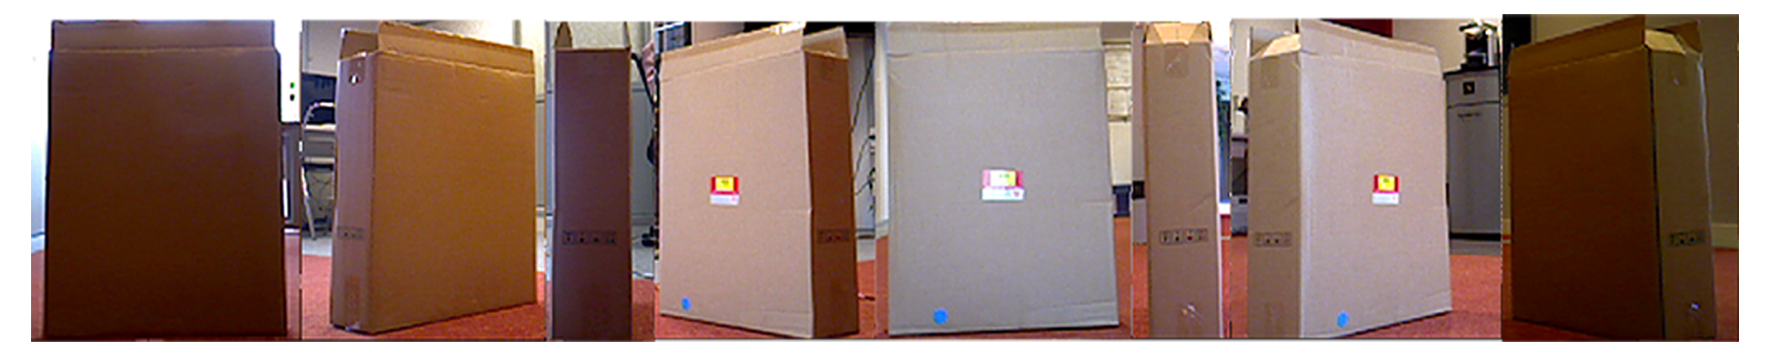
\includegraphics[width=\textwidth]{box_seq.png}}
\end{figure}

\begin{figure}[H]
	\subfloat{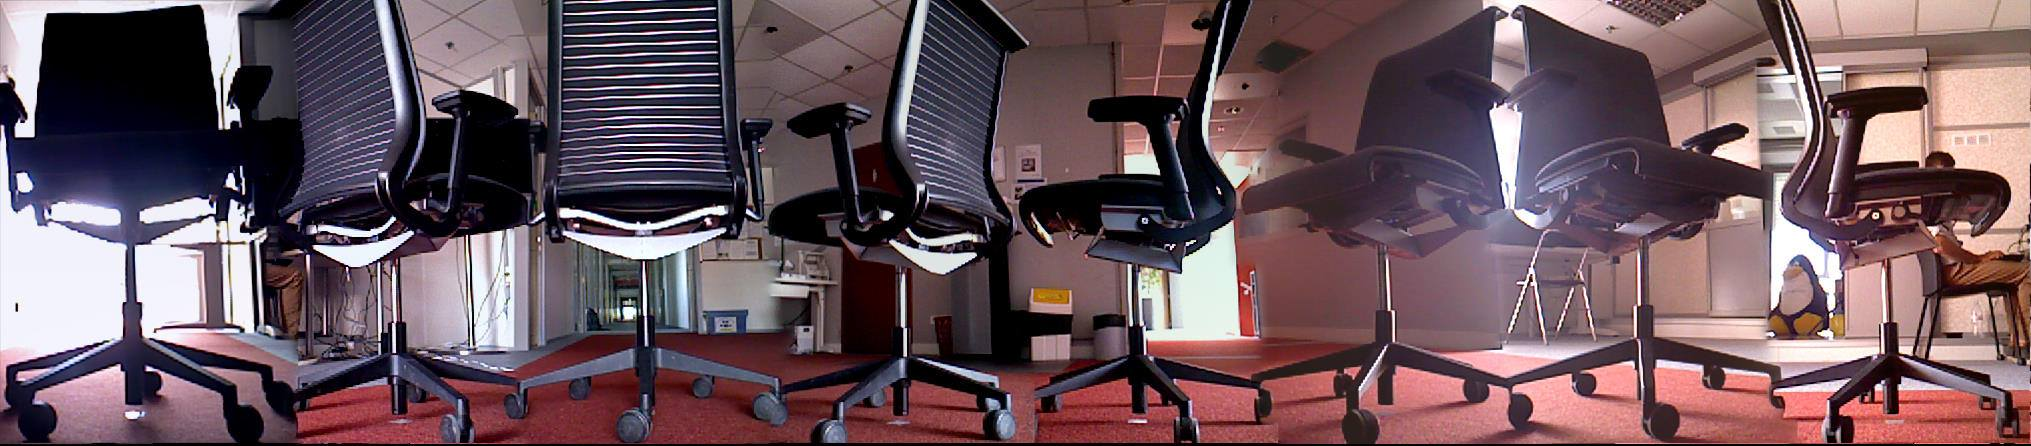
\includegraphics[width=\textwidth]{chair_db.jpg}}
\end{figure}

\begin{figure}[H]
	\subfloat{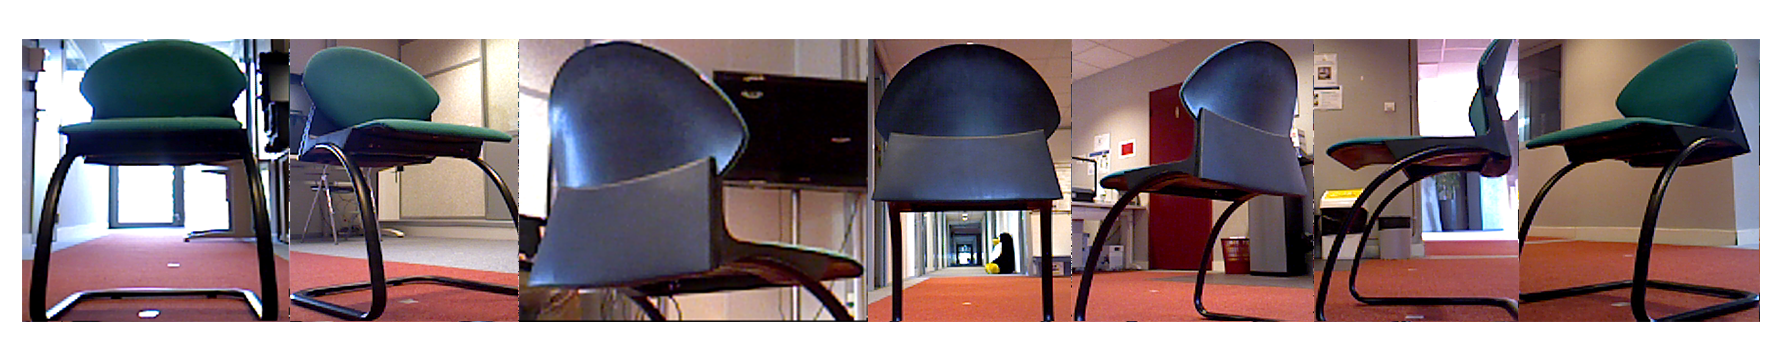
\includegraphics[width=\textwidth]{chair_seq.png}}
\end{figure}

\begin{figure}[H]
	\subfloat{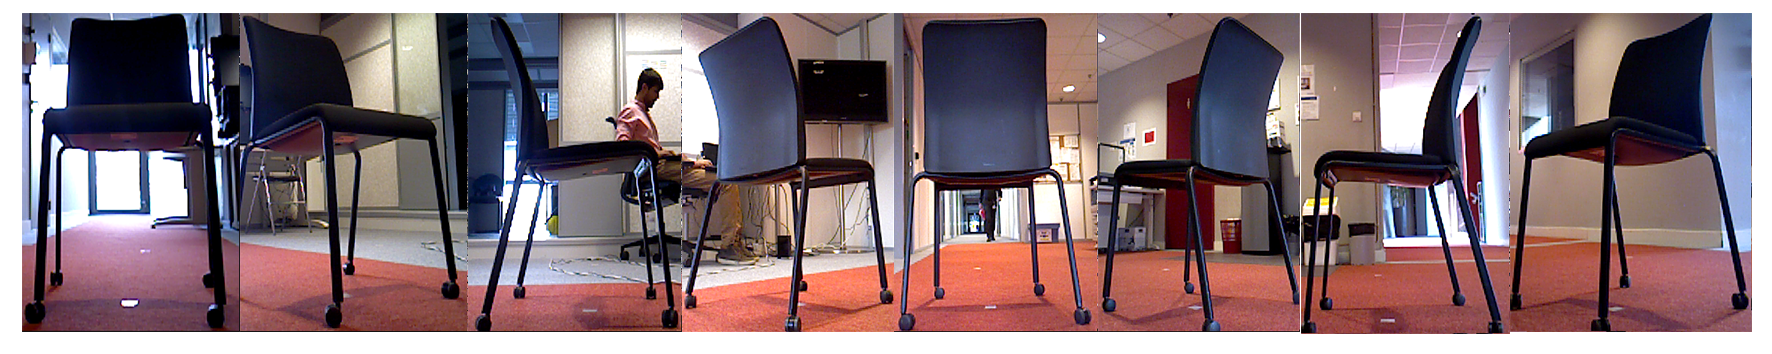
\includegraphics[width=\textwidth]{chair4w.png}}			
\end{figure}

\subsection{Estimation de la normale}

Pour constituer les informations géométriques l'estimation de la normale du point est d'extrême importance. 

Sont calcul est fait de la manière suivant :
1. Un nombre de voisins est choisi 
2. Ces point *servem* à trouver des paramètres de l'équation du plan tangent et, par consequent, la normale correspondent.

Le méthode adopté pour la bibliothéque PCL correspond à prendre un certain nombre de plus proches voisins définis par un seiul. Un petit seil rendre le calcul faux et un grand prend en compte points distants que peuvent ne pas faire partie du plan estimé.

\url{http://www.pointclouds.org/documentation/tutorials/vfh_recognition.php#vfh-recognition} \\

\url{http://pointclouds.org/documentation/tutorials/fpfh_estimation.php} \\

\url{https://github.com/PointCloudLibrary/pcl/wiki/Overview-and-Comparison-of-Features} \\

\subsection { RANSAC } 

The RANSAC algorithm is a learning method to estimate a given model parameters. Contrary to other estimation algorithms, which considers the whole data represenetative to model estimation, RANSAC suppose the existance of \textbf{inliers or consensus} and \textbf{outliers}  and uses a voting scheme to select between reliable data, that must follow two assumptions: 

\begin{itemize}
  \item Noisy data will not vote consistenly for a single model - (few outliners) 
  \item Enough good features voting for the same model - (few missing data)
\end{itemize}

\subsubsection{The RANSAC algorithm}

The iterative algorithm is composed of two different stages : 
\begin {itemize}
  \item Sample minimal data from dataset requerid to first estimate model parameters.
  \item Given a threshold error, it selects data points that are consistent to the model created in the first step.
\end {itemize}

\begin{itemize}
  \item Random hypoythetical inliers subset
  \item Find model parameters
  \item All data tested according to a loss function that determine the \textit{consensus}
  \item Finishes when a sufficient number of point belongs to the \textit{consensus}
\end{itemize}

\center \large{\color{blue} If the variables are linear and normally distributed the Bayes filter becomes equal to the Kalman filter.}

%% \caption{My algorithm}\label{euclid}
%%     \begin{algorithmic}[1]
%%         \Procedure{RANSAC}{}
%%         \State $\textit{stringlen} \gets \text{length of }\textit{string}$
%%         \State $i \gets \textit{patlen}$
%%         \BState \emph{top}:
%%         \If {$i > \textit{stringlen}$} \Return false
%%         \EndIf
%%         \State $j \gets \textit{patlen}$
%%         \BState \emph{loop}:
%%         \If {$\textit{string}(i) = \textit{path}(j)$}
%%         \State $j \gets j-1$.
%%         \State $i \gets i-1$.
%%         \State \textbf{goto} \emph{loop}.
%%         \State \textbf{close};
%%         \EndIf
%%         \State $i \gets i+\max(\textit{delta}_1(\textit{string}(i)),\textit{delta}_2(j))$.
%%         \State \textbf{goto} \emph{top}.
%%         \EndProcedure
%%     \end{algorithmic}
%% \end{algorithm}


\textit{L'Universidad de León } a fait un compte rendu des
\textit{features} implementés sur PCL dans le lien *[8]*. Plus
d'information sur les descripteur et ses implementations sur la
librarie PCL peuvent être retrouvés sur le site
internet \url{http://pointclouds.org}.

Les images sont sauvegardées à l'aide de la librarie OpenCv dans le format 8\_U et .png (Portable Network Graphics).

Les nauges de points sont sauvegardées dans le format .pcd (Point Cloud Data).

Pour sauvegarder les information *provenientes* de la segmentation, les [it]topics de sorti sont souscrit avec rosbag pendent le deplacement du robot. Les messages sauvegardes sont le suivants :

\begin{itemize}
\item v\_objects\_clouds : Vector de nuages de points obtenues pour chaque objet 

\item v\_objects\_image\_and\_mask : Sousimages et mask de chaque objet

\item v\_object\_

\end{itemize}


\section{Planning de Travail}
\begin{itemize}
    \item[\checkmark] Mise en place de l'architecture et des protocoles de communication entre composants physiques.
    \item[\checkmark] Étude bibliographique initiale pour situer le travail par rapport à l'existant.
    \item[\checkmark] Implémentation de l'asservissement d'une caméra PTZ par rapport au retour d'un algorithme de tracking.
    \item[\checkmark] Aperçu de certaines limitations de la caméra PTZ qui a été remplacée par une caméra RGB-D.
    \item[\checkmark] Utilisation d'un algorithme de segmentation d'objets possibles dans la scène.
    \item[\checkmark] Asservissement en boucle ouvert du robot pour la création de la base de données.
    \item[\checkmark] Premiers tests pour l'acquisition de la base des données.
    \item Résolution des problèmes trouvés lors des premiers tests pour la création de la base de données.
    \item Validation de la base de données. Représentativité et reproduction.
    \item Étude approfondie de l’état de l'art des modèles et méthodes qui puissent être utiles pour notre problème.
    \item Mise en place de la solution et du modèle proposé.
    \item Premiers tests et ajustements nécessaires.
    \item Mise en œuvre de la solution complète.
    \item Validation finale.    
\end{itemize}
